% *********************************************************************
% © 2010–2023 Jeremy Sylvestre
%
% Permission is granted to copy, distribute and/or modify this document
% under the terms of the GNU Free Documentation License, Version 1.3 or
% any later version published by the Free Software Foundation; with no
% Invariant Sections, no Front-Cover Texts, and no Back-Cover Texts. A
% copy of the license is included in the appendix entitled “GNU Free
% Documentation License” that appears in the output document of this
% PreTeXt source code. All trademarks™ are the registered® marks of
% their respective owners.
%
% *********************************************************************

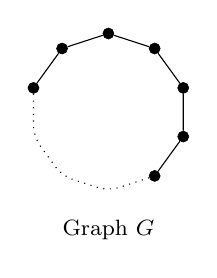
\begin{tikzpicture}[
	vertex/.style={ circle, draw, very thin, fill, inner sep=0pt, minimum size=4pt },
	vertexg/.style={ black!40!white, circle, draw, very thin, fill, inner sep=0pt, minimum size=4pt },
	vertexo/.style={ circle, draw, very thin, inner sep=0pt, minimum size=4pt }
]

\node[vertex] at (0,1) (v1) {};
\node[vertex] at (0.588,0.809) (v2) {};
\node[vertex] at (0.951,0.309) (v3) {};
\node[vertex] at (0.951,-0.309) (v4) {};
\node[vertex] at (0.588,-0.809) (v5) {};
\node[vertex] at (-0.588,0.809) (vn) {};
\node[vertex] at (-0.951,0.309) (vnm1) {};
\draw (vnm1) to (vn) to (v1) to (v2) to (v3) to (v4) to (v5);
%\draw[dotted] (v5) .. controls (0.044,-1.559) and (-1.496,-0.441) .. (vnm1);
\draw[dotted,rounded corners]
  (v5)
  to (0,-1)
  to (-0.588,-0.809)
  to (-0.951,-0.309)
  to (vnm1);
\node at (0,-1.5) {\footnotesize Graph $G$};

\end{tikzpicture}
